\def\sclI{4.15}
\def\panelw{7.4}
\def\panelh{5.4}

\definecolor{tfd1face}{HTML}{97F4EB}
\definecolor{tfd1edge}{HTML}{0D665C}
\definecolor{tfd2face}{HTML}{008777}
\definecolor{tfd2edge}{HTML}{063A33}
\definecolor{tfrface}{HTML}{C8467A}
\definecolor{tfredge}{HTML}{5A1F36}
\definecolor{tfvedot}{HTML}{5A1F36}
\definecolor{tfbg}{HTML}{ECECEE}

\newcommand{\proj}[3]{%
  ({((#1) * 0.7880107536 + (#2) * 0.6156614753) * \sclI},
   {((#1) * (-0.1901783216) + (#2) * 0.2433065857 + (#3) * 0.9510565163) * \sclI - 0.35})%
}

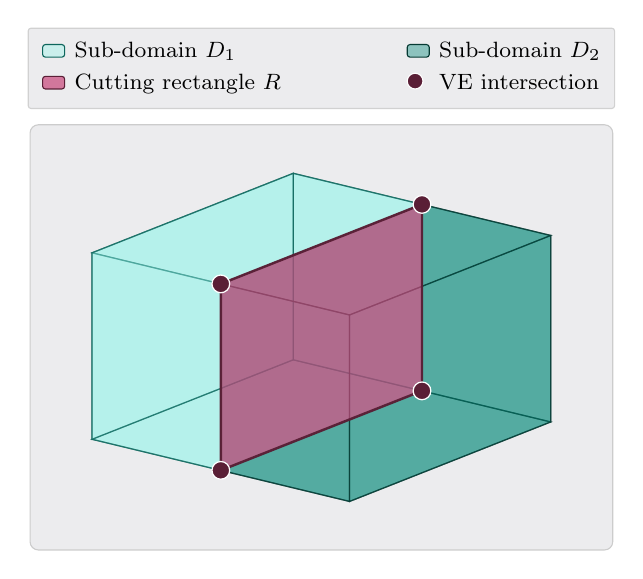
\begin{tikzpicture}[font=\sffamily\footnotesize, x=1cm, y=1cm]

  \filldraw[
    fill=tfbg,
    draw=black!20,
    line width=0.4pt,
    rounded corners=3pt
  ]
    (-\panelw/2, -\panelh/2 - 0.35) rectangle (\panelw/2, \panelh/2 - 0.35);

  % --------------------------------------------------------------------
  % D1 outer faces
  % --------------------------------------------------------------------

  \filldraw[
    fill=tfd1face,
    draw=tfd1edge,
    fill opacity=0.40,
    draw opacity=0.75,
    line width=0.45pt
  ]
    \proj{-0.5}{-0.5}{-0.3}
    -- \proj{0}{-0.5}{-0.3}
    -- \proj{0}{0.5}{-0.3}
    -- \proj{-0.5}{0.5}{-0.3}
    -- cycle;

  \filldraw[
    fill=tfd1face,
    draw=tfd1edge,
    fill opacity=0.40,
    draw opacity=0.75,
    line width=0.45pt
  ]
    \proj{-0.5}{-0.5}{0.3}
    -- \proj{0}{-0.5}{0.3}
    -- \proj{0}{0.5}{0.3}
    -- \proj{-0.5}{0.5}{0.3}
    -- cycle;

  \filldraw[
    fill=tfd1face,
    draw=tfd1edge,
    fill opacity=0.40,
    draw opacity=0.75,
    line width=0.45pt
  ]
    \proj{-0.5}{-0.5}{-0.3}
    -- \proj{0}{-0.5}{-0.3}
    -- \proj{0}{-0.5}{0.3}
    -- \proj{-0.5}{-0.5}{0.3}
    -- cycle;

  \filldraw[
    fill=tfd1face,
    draw=tfd1edge,
    fill opacity=0.40,
    draw opacity=0.75,
    line width=0.45pt
  ]
    \proj{0}{0.5}{-0.3}
    -- \proj{-0.5}{0.5}{-0.3}
    -- \proj{-0.5}{0.5}{0.3}
    -- \proj{0}{0.5}{0.3}
    -- cycle;

  \filldraw[
    fill=tfd1face,
    draw=tfd1edge,
    fill opacity=0.40,
    draw opacity=0.75,
    line width=0.45pt
  ]
    \proj{-0.5}{-0.5}{-0.3}
    -- \proj{-0.5}{0.5}{-0.3}
    -- \proj{-0.5}{0.5}{0.3}
    -- \proj{-0.5}{-0.5}{0.3}
    -- cycle;

  % --------------------------------------------------------------------
  % D2 outer faces
  % --------------------------------------------------------------------

  \filldraw[
    fill=tfd2face,
    draw=tfd2edge,
    fill opacity=0.40,
    draw opacity=0.75,
    line width=0.45pt
  ]
    \proj{0}{-0.5}{-0.3}
    -- \proj{0.5}{-0.5}{-0.3}
    -- \proj{0.5}{0.5}{-0.3}
    -- \proj{0}{0.5}{-0.3}
    -- cycle;

  \filldraw[
    fill=tfd2face,
    draw=tfd2edge,
    fill opacity=0.40,
    draw opacity=0.75,
    line width=0.45pt
  ]
    \proj{0}{-0.5}{0.3}
    -- \proj{0.5}{-0.5}{0.3}
    -- \proj{0.5}{0.5}{0.3}
    -- \proj{0}{0.5}{0.3}
    -- cycle;

  \filldraw[
    fill=tfd2face,
    draw=tfd2edge,
    fill opacity=0.40,
    draw opacity=0.75,
    line width=0.45pt
  ]
    \proj{0}{-0.5}{-0.3}
    -- \proj{0.5}{-0.5}{-0.3}
    -- \proj{0.5}{-0.5}{0.3}
    -- \proj{0}{-0.5}{0.3}
    -- cycle;

  \filldraw[
    fill=tfd2face,
    draw=tfd2edge,
    fill opacity=0.40,
    draw opacity=0.75,
    line width=0.45pt
  ]
    \proj{0.5}{0.5}{-0.3}
    -- \proj{0}{0.5}{-0.3}
    -- \proj{0}{0.5}{0.3}
    -- \proj{0.5}{0.5}{0.3}
    -- cycle;

  \filldraw[
    fill=tfd2face,
    draw=tfd2edge,
    fill opacity=0.40,
    draw opacity=0.75,
    line width=0.45pt
  ]
    \proj{0.5}{-0.5}{-0.3}
    -- \proj{0.5}{0.5}{-0.3}
    -- \proj{0.5}{0.5}{0.3}
    -- \proj{0.5}{-0.5}{0.3}
    -- cycle;

  % --------------------------------------------------------------------
  % Cutting rectangle R
  % --------------------------------------------------------------------

  \filldraw[
    fill=tfrface,
    draw=tfredge,
    fill opacity=0.70,
    draw opacity=0.95,
    line width=0.9pt
  ]
    \proj{0}{-0.5}{-0.3}
    -- \proj{0}{0.5}{-0.3}
    -- \proj{0}{0.5}{0.3}
    -- \proj{0}{-0.5}{0.3}
    -- cycle;

  % --------------------------------------------------------------------
  % VE intersection points
  % --------------------------------------------------------------------

  \foreach \x/\y/\z in {
    0/-0.5/-0.3,
    0/0.5/-0.3,
    0/0.5/0.3,
    0/-0.5/0.3
  }{
    \filldraw[
      fill=tfvedot,
      draw=white,
      line width=0.45pt
    ] \proj{\x}{\y}{\z} circle [radius=3.2pt];
  }

  % --------------------------------------------------------------------
  % Legend above drawing
  % --------------------------------------------------------------------

  \node[
    anchor=south,
    fill=tfbg,
    draw=black!18,
    rounded corners=1pt,
    inner xsep=5pt,
    inner ysep=4pt,
    font=\footnotesize,
    minimum width=\panelw cm
  ] at (0, 2.55)
  {
    \begin{tabular}{@{}l@{\hspace{0.4em}}l@{\hspace{1.6cm}}l@{\hspace{0.4em}}l@{}}
      \tikz{\draw[fill=tfd1face, draw=tfd1edge, fill opacity=0.40] (0,0) rectangle (0.28,0.16);}
      &
      Sub-domain $D_1$
      &
      \tikz{\draw[fill=tfd2face, draw=tfd2edge, fill opacity=0.40] (0,0) rectangle (0.28,0.16);}
      &
      Sub-domain $D_2$
      \\[2pt]
      \tikz{\draw[fill=tfrface, draw=tfredge, fill opacity=0.70] (0,0) rectangle (0.28,0.16);}
      &
      Cutting rectangle $R$
      &
      \tikz{\filldraw[fill=tfvedot, draw=white, line width=0.4pt] (0.14,0.08) circle (0.10);}
      &
      VE intersection
    \end{tabular}
  };

\end{tikzpicture}
